
% Template for Elsevier CRC journal article
% version 1.2 dated 09 May 2011

% This file (c) 2009-2011 Elsevier Ltd.  Modifications may be freely made,
% provided the edited file is saved under a different name

% This file contains modifications for Procedia Computer Science
% but may easily be adapted to other journals

% Changes since version 1.1
% - added "procedia" option compliant with ecrc.sty version 1.2a
%   (makes the layout approximately the same as the Word CRC template)
% - added example for generating copyright line in abstract

%-----------------------------------------------------------------------------------

%% This template uses the elsarticle.cls document class and the extension package ecrc.sty
%% For full documentation on usage of elsarticle.cls, consult the documentation "elsdoc.pdf"
%% Further resources available at http://www.elsevier.com/latex

%-----------------------------------------------------------------------------------

%%%%%%%%%%%%%%%%%%%%%%%%%%%%%%%%%%%%%%%%%%%%%%%%%%%%%%%%%%%%%%
%%%%%%%%%%%%%%%%%%%%%%%%%%%%%%%%%%%%%%%%%%%%%%%%%%%%%%%%%%%%%%
%%                                                          %%
%% Important note on usage                                  %%
%% -----------------------                                  %%
%% This file should normally be compiled with PDFLaTeX      %%
%% Using standard LaTeX should work but may produce clashes %%
%%                                                          %%
%%%%%%%%%%%%%%%%%%%%%%%%%%%%%%%%%%%%%%%%%%%%%%%%%%%%%%%%%%%%%%
%%%%%%%%%%%%%%%%%%%%%%%%%%%%%%%%%%%%%%%%%%%%%%%%%%%%%%%%%%%%%%

%% The '3p' and 'times' class options of elsarticle are used for Elsevier CRC
%% Add the 'procedia' option to approximate to the Word template
%\documentclass[3p,times,procedia]{elsarticle}
\documentclass[3p,times]{elsarticle}

%% The `ecrc' package must be called to make the CRC functionality available
\usepackage{ecrc}
\usepackage{xcolor}

%% The ecrc package defines commands needed for running heads and logos.
%% For running heads, you can set the journal name, the volume, the starting page and the authors

%% set the volume if you know. Otherwise `00'
\volume{00}

%% set the starting page if not 1
\firstpage{1}

%% Give the name of the journal
\journalname{Procedia Computer Science}
\runauth{}
\jid{procs}

%% Give a short journal name for the dummy logo (if needed)
\jnltitlelogo{Procedia Computer Science}
\CopyrightLine{2011}{Published by Elsevier Ltd.}
%%%%%%%%%%%%%%%%%%%%%%%%%%%%%%%%%%%%%%%%%%%%%%%%%%%%%%%%%%%%%%%%%%%%%%%%%%

\usepackage{amssymb}
\usepackage[figuresright]{rotating}
\usepackage{float}
\usepackage{lscape}
\usepackage{xltabular}
\usepackage{array} 
\usepackage{tabularx}
\usepackage{ragged2e}
\usepackage{longtable}
\usepackage{geometry}
\usepackage{xltabular}

\usepackage{graphicx}
\usepackage{subcaption}
\usepackage[export]{adjustbox}
\usepackage{wrapfig}
\usepackage[rightcaption]{sidecap}
\usepackage{hyperref}

\begin{document}

\begin{frontmatter}

%% Title, authors and addresses

%% use the tnoteref command within \title for footnotes;
%% use the tnotetext command for the associated footnote;
%% use the fnref command within \author or \address for footnotes;
%% use the fntext command for the associated footnote;
%% use the corref command within \author for corresponding author footnotes;
%% use the cortext command for the associated footnote;
%% use the ead command for the email address,
%% and the form \ead[url] for the home page:
%%
%% \title{Title\tnoteref{label1}}
%% \tnotetext[label1]{}
%% \author{Name\corref{cor1}\fnref{label2}}
%% \ead{email address}
%% \ead[url]{home page}
%% \fntext[label2]{}
%% \cortext[cor1]{}
%% \address{Address\fnref{label3}}
%% \fntext[label3]{}

\dochead{}
%% Use \dochead if there is an article header, e.g. \dochead{Short communication}
%% \dochead can also be used to include a conference title, if directed by the editors
%% e.g. \dochead{17th International Conference on Dynamical Processes in Excited States of Solids}

\title{BlockEstate: Revolutionizing Real Estate Transactions through Hyperledger-Based Blockchain Technology}

%% use optional labels to link authors explicitly to addresses:
\author[label1]{Laviza Falak Naz}%
%\author[label1]{Author 2}
%\author[label2]{Author 3}
\address[label1]{NED University of Engineering \& Technology}
%\address[label2]{Affiliation 2}

\begin{abstract}

This paper presents BlockEstate, a state of the art stage for land exchanges in view of the Hyperledger blockchain design. With the presentation of a progressive compensation request instrument and an unmistakable chaincode for overseeing property possession, BlockEstate changes the traditional land exchange method. The stage uses the decentralization, unchanging nature, and straightforwardness of blockchain innovation to handle the normal failures and security issues in land exchanges. The compensation request technique ensures protected and straightforward monetary exchanges, while the chaincode mechanizes the exchange of property possession. This study takes a gander at the plan, activity, and utilization of BlockEstate. It likewise examinations the security and protection angles exhaustively and takes a gander at the troubles and limitations that accompany utilizing blockchain innovation in the land business. BlockEstate's convenience is shown through an imaginary contextual investigation that underlines the stage's security, viability, and potential to change the land business. The potential for blockchain innovation in land and the impact of sites like BlockEstate on this improvement are canvassed in the paper's decision.

\end{abstract}

\begin{keyword}
%% keywords here, in the form: keyword \sep keyword
%% PACS codes here, in the form: \PACS code \sep code
%% MSC codes here, in the form: \MSC code \sep code
%% or \MSC[2008] code \sep code (2000 is the default)
Blockchain Technology \sep Real Estate Transactions \sep Hyperledger Framework \sep Chaincode \sep Property Ownership Management \sep Pay Order Mechanism \sep Decentralization \sep Transaction Security \sep Financial Transparency \sep Smart Contracts \sep Digital Tokenization \sep Property Token
\end{keyword}

\end{frontmatter}

%%
%% Start line numbering here if you want
%%
% \linenumbers

%% main text
\section{Introduction}

The emergence of blockchain technology has sparked a new era of innovation that has not gone unnoticed in the real estate sector. Long cycles, an absence of straightforwardness, and a critical gamble of extortion are among of the issues that plague customary land exchanges \cite{saari2022blockchain}. These troubles require areas of strength for a that guarantees security and straightforwardness while smoothing out exchanges. The revolutionary real estate transaction platform BlockEstate, which is built on the Hyperledger blockchain, is discussed in this article. BlockEstate is altering land exchanges by using the inherent benefits of blockchain innovation, including permanence, decentralization, and straightforwardness \cite{garcia2020legal}. The stage utilizes an extraordinary chaincode to follow property proprietorship, which is upheld by another compensation request framework that makes property exchanges safer and effective.

The plan of BlockEstate gives a far reaching answer for the current failures in the housing market. It guarantees that all exchanges are noticeable and irreversible by permitting a decentralized record framework. The stage's chaincode is particularly worked to follow property possession, while the compensation request framework guarantees protected and straightforward monetary exchanges among purchasers and dealers \cite{ullah2023conceptual}. The reason for this paper is to make sense of the working, benefits, and conceivable impact of BlockEstate in land exchange change.

\section{Related Work}

Ongoing scholar and industry study \cite{podshivalov2022improving} has shown a rising interest in the utilization of blockchain innovation in land. A few examinations have underscored blockchain's true capacity in handling huge challenges in land exchanges, like extortion, absence of straightforwardness, and shortcomings, \cite{wouda2019blockchain}. The qualities of blockchain, especially its decentralized nature and sealed record, have been featured as basic in working on the dependability and effectiveness of land exchanges \cite{latifi2019blockchain}.

Earlier blockchain involves in land have for the most part centered around digitizing property records and smoothing out title moves, as per \cite{konashevych2020constraints}. These frameworks, notwithstanding, every now and again needed total answers for exchange the executives and monetary security, which are pivotal in land exchanges. Savvy contracts have as of late been acquainted with robotize exchange methods \cite{veuger2020dutch}, however the intricacy of land exchanges, spreading over lawful, monetary, and administrative issues, requires a more customized arrangement \cite{jeong2021implementation}.

The BlockEstate arrangement, which utilizes Hyperledger's secluded and versatile construction, denotes a significant jump in this area \cite{mittal2020real}. Due to Hyperledger's adaptability for private exchanges and adaptable agreement techniques, it is appropriate for land applications where security and proficiency are basic \cite{gupta2020tokenization}. In contrast with regular brilliant agreements, the stage's chaincode for property proprietorship the executives gives a more complex and versatile arrangement, addressing especially to the different idea of land exchanges \cite{huh2020verification}.

Besides, BlockEstate's compensation request component fills a huge need in existing blockchain land frameworks, \cite{pankratov2020blockchain}. While past models gave a protected record to property data, they much of the time missed the intricacies of land monetary exchanges. BlockEstate's mediation ledger concept not only ensures the security of financial transactions, but it also provides a transparent and reversible transaction process, boosting buyer and seller confidence.

All in all, while blockchain innovation has been concentrated on with regards to land exchanges, BlockEstate's imaginative use of Hyperledger and its remarkable compensation request component fill a significant hole in the current exploration and practice. The purpose of this study is to demonstrate how BlockEstate can revolutionize real estate transactions and set a new standard for how blockchain technology is used in the industry.

\section{BlockEstate Architecture}

BlockEstate is a pivotal land exchange stage based on serious areas of strength for the versatile Hyperledger blockchain \cite{bhanushali2020blockchain} system. The architecture of BlockEstate is specifically designed to adapt to the subtleties and complexity of real estate transactions, offering a safe, transparent, and effective solution (cite Konashevych, 2020 general). The decentralized record at the core of BlockEstate's plan empowers for the permanent recording of property exchanges, helping trust and straightforwardness all the while.


The functionality of BlockEstate is contingent on the utilization of Hyperledger as the underlying technology. As opposed to public blockchains, Hyperledger gives a permissioned network climate, which is basic for safeguarding secrecy in land exchanges. It makes it possible to set up private channels, allowing specific data to be shared only with authorized parties, which is crucial when dealing with sensitive information in real estate transactions.


\subsection{Network Structure}

BlockEstate's organization structure is comprised of numerous hubs, every one of which addresses a particular player in the housing market, like purchasers, merchants, monetary establishments, and administrative associations \cite{ferreira2021blockchain}. These hubs take part in the agreement cycle, guaranteeing exchange authenticity and realness. The plan additionally contains savvy contracts or chaincode, which mechanize exchange methods and implement the BlockEstate \cite{hoxha2019study} business rules.


\subsection{Chaincode for Property Ownership}

The chaincode intended for property possession the board is a significant piece of the design. This chaincode oversees and confirms possession moves as a computerized transitional. It ensures that all property data is correctly captured and stored on the blockchain "cite mehendale2019implications." Besides, the chaincode improves on the execution of convoluted exchanges, for example, property tokenization, which carefully considers land resources the blockchain.


\begin{figure}[H]
    \centering
    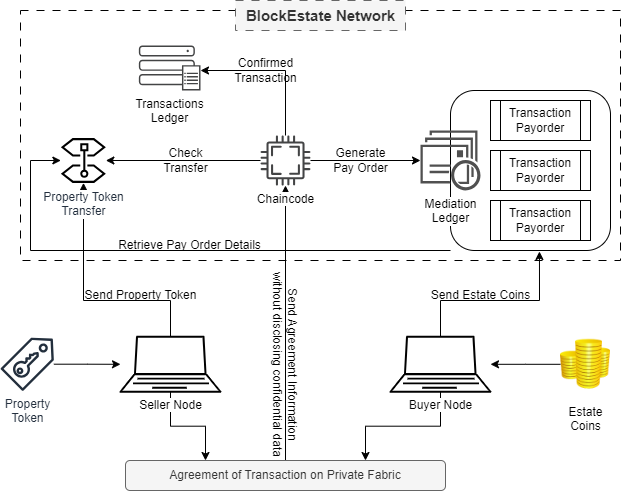
\includegraphics[width=1\linewidth]{images/Bllockchain.drawio.png}
    \caption{BlockEstate Architecture diagram}
    \label{fig:fig1}
\end{figure}


\section{Pay Request Mechanism}

The BlockEstate pay request strategy is a creative procedure to managing monetary exchanges in the housing market. This procedure is basic for keeping up with monetary security and straightforwardness in land exchanges.

\subsection{Functionality}

At the point when a property exchange is begun, the purchaser's cash are not moved directly to the dealer. All things considered, they are recorded as a compensation request in an intervention record. The buyer and seller "citeavantaggiato2019challenges" are the only people who have access to the transaction information in this ledger, which is accessible to all network peers. However, this ledger does not permit access to private data.


\subsection{Security and Transparency}

The intervention record fills in as a protected store box for exchange monies. It catches all exchange information while ensuring that private data is kept mystery. This technique defends the money as well as guarantees straightforwardness for all gatherings taking part in the exchange \cite{citesladic2021blockchain}.

\subsection{Automated Affirmation and Reversion}

The chaincode is basic to the compensation request methodology. The chaincode consequently approves the compensation request in the intervention record and disseminates the money to the dealer upon the exchange of the property token from the merchant to the purchaser. This mechanization ensures that the progression of installments is contingent on the effective exchange of property proprietorship, \cite{mashatan2021usurping}. The pay order is canceled and the funds are returned to the buyer if the property token is not transferred within the specified time frame. This element offers a level of monetary security, safeguarding the two players' inclinations.

\begin{figure}[H]
    \centering
    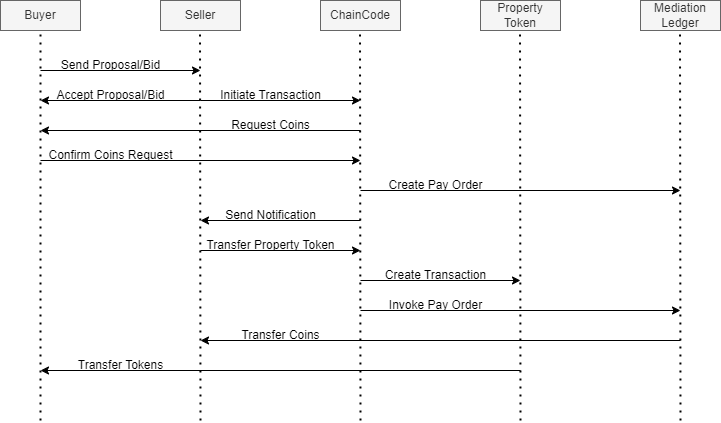
\includegraphics[width=1\linewidth]{images/state flow diagram.drawio.png}
    \caption{BlockEstate transaction flow diagram}
    \label{fig:fig2}
\end{figure}

At last, the BlockEstate design, upheld by the Hyperledger structure, and its original compensation request component joined set another norm in land exchanges. The blend of these innovations handles a large number of the current land challenges, giving a framework that isn't just more productive and safe, yet additionally straightforward and easy to use \cite{harris2021blockchain}.

\section{Chaincode Functionality}

The chaincode, a basic part of BlockEstate's plan, goes about as the stage's conditional spine. Basically an assortment of programmable directions run on the Hyperledger blockchain and are intended to oversee and work with land exchanges.

\begin{verbatim}
Pseudocode for BlockEstate Chaincode

// Initialization of the chaincode
Initialize Chaincode
    Initialize ledger state

// Handler for various chaincode invocations
Invoke Function

// Create a new property record
CreateProperty(property details)
    Validate property details, Store property in ledger, Return success or error message

// Transfer property ownership
TransferProperty(property ID, new owner)
    Retrieve property from ledger, Verify ownership and transfer conditions, 
    Update property record with new owner, Return success or error message

// Create a pay order for a property transaction
CreatePayOrder(buyer, seller, amount)
    Validate transaction details, Create and store pay order in ledger, 
    Lock transaction amount in mediation ledger, Return success or error message

// Confirm a pay order upon successful property transfer
ConfirmPayOrder(pay order ID)
    Retrieve pay order from ledger, Verify property transfer completion,
    Update pay order status, Transfer funds from mediation ledger to seller, 
    Return success or error message

\end{verbatim}

\subsection{Technical Implementation}

The chaincode in BlockEstate is written in a significant level programming language upheld by the Hyperledger Texture structure, for example, Go or JavaScript. This programming style empowers the advancement of mind boggling business rationale to oversee numerous components of property exchanges \cite{veuger2020database}. The guidelines for validating transactions, executing pay orders, and transferring ownership of property are all contained in the chaincode.


\subsection{Property Possession Management}

One of the chaincode's key liabilities is to safely and really handle property possession records. At the point when a property is posted on the BlockEstate stage, the chaincode makes an exceptional computerized token to address it. This token is safe-stored on the blockchain citehermansson2020real and provides crucial property facts like location, size, and legal information.

\subsection{Transaction Interaction Automation}

The chaincode smoothes out the purchaser vender exchange technique. The chaincode checks the accessibility and responsibility for property token when an exchange is sent off. It then, at that point, administers the compensation request framework, guaranteeing that monies are securely kept in the intercession record until the deal's all's models are fulfilled \cite{saull2020can}.

\subsection{Ensuring Consistence and Security}

The chaincode's programmability guarantees that all exchanges comply with preset principles and limitations \cite{lindholm2021blockchain}. It additionally plays a significant capability in guaranteeing exchange security by forestalling unapproved access and deceitful movement.

\section{Case Study/Application Example}

An imagined contextual investigation is proposed to show the reasonable execution and advantages of BlockEstate.

\subsection{Background}

Think about the accompanying situation: a purchaser, Alice, wishes to buy a home from a vender, Weave. The property is posted on the BlockEstate stage \cite{li2019blockchain} and is situated in an extraordinary metropolitan district.

\subsection{Initiation of Transaction}

On the BlockEstate stage, Alice begins the exchange. The chaincode produces a compensation request because of her sign of interest, defending the exchange sum in the intervention record.

Subsection Token Transfer and Pay Order Confirmation: Bob transfers Alice's property token through the BlockEstate platform. The chaincode approves the exchange and affirms the compensation request consequently. Bounce \cite{hutson2023architecting} gets the monies from the intercession record.

\subsection{Efficiency and Security Benefits}

This contextual analysis features BlockEstate's productivity and security benefits. The exchange system is improved, which diminishes the time and intricacy associated with common land exchanges. Besides, the chaincode and pay request instrument \cite{bhatia2019exploration} guarantee the security of cash and the straightforwardness of the exchange.

\begin{figure}[H]
    \centering
    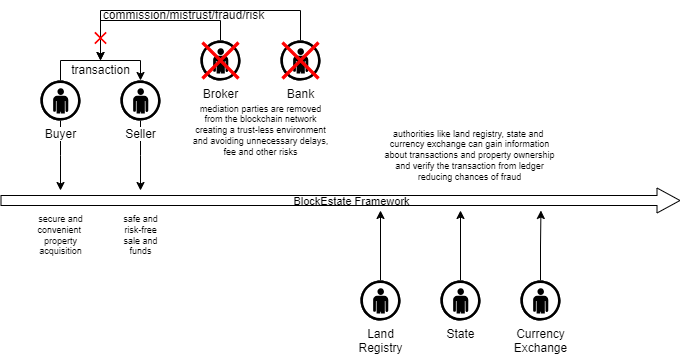
\includegraphics[width=1.0\linewidth]{images/use case.drawio.png}
    \caption{Application of BlockEstate Framework in Real Estate Market}
    \label{fig:fig3}
\end{figure}

At last, as exhibited by the contextual investigation, the BlockEstate stage, with its clever utilization of chaincode and the compensation request instrument, gives a more productive, safe, and straightforward methodology for land exchanges.

Section Security and Privacy Considerations BlockEstate has demonstrated that the use of blockchain technology in real estate transactions significantly enhances security and privacy. However, these developments necessitate a comprehensive examination of the associated risks and approaches to mitigation. \cite{kothari2020smart}.

\subsection{Data Encryption and Access Control}

Delicate information, as purchaser and merchant individual data and property token particulars, is scrambled in BlockEstate. Advanced encryption algorithms can be used to protect data both in transit and at rest thanks to the Hyperledger framework. Moreover, access control measures are utilized to ensure that main approved clients approach specific information, subsequently safeguarding protection.

\subsection{Smart Agreement Security}

BlockEstate's chaincode, or shrewd agreements, are broadly tried to stay away from weaknesses that might be manhandled \cite{baum2021tokenization}. The convention incorporates normal reviews and moves up to protect the chaincode's trustworthiness and security, thus defending the stage from potential breaks or deceitful action.

\subsection{Regulatory Compliance}

BlockEstate is planned to conform to existing land and information insurance rules, as per \cite{moringiello2022blockchain}. The stage follows administrative prerequisites for information security, like GDPR, and nearby land regulation, it are mechanically protected as well as lawfully sound to ensure that exchanges.

\section{Challenges and Limitations}

Regardless of BlockEstate's imaginative methodology and prevalent innovation, there are intrinsic obstructions and limits that should be perceived \cite{tilbury2019business}.

\subsection{Technical Complexity}

The utilization of blockchain innovation in land is in fact testing. The creation and upkeep of the BlockEstate stage require impressive specialized information, strikingly in blockchain innovation and brilliant agreement programming \cite{jain2020blockchain}.

\subsection{Adoption and Integration}

Reception of blockchain innovation offers a major test in the ordinarily safe housing market. While coordinating BlockEstate with current land cycles and frameworks, resistance and specialized similarity difficulties might emerge \cite{yacob2021blockchain}.

\subsection{Scalability and Performance}

Adaptability and execution are potential cutoff points, as they are with numerous blockchain innovations. It is basic for BlockEstate's drawn out endurance to guarantee that it can deal with a colossal volume of exchanges without forfeiting velocity or proficiency.

\section{Conclusion}

BlockEstate is a major step in the right direction in the utilization of blockchain innovation for land exchanges. Using the Hyperledger foundation and introducing a novel pay order system, BlockEstate addresses significant issues in the real estate market, such as transaction inefficiencies, a lack of transparency, and security concerns.

The stage's original plan and chaincode abilities increment the productivity, security, and straightforwardness of land exchanges, \cite{shuaib2021improving}. While there are sure limits and obstacles, for example, specialized intricacy and versatility issues, the expected advantages of BlockEstate in reforming land exchanges are obvious.

As blockchain innovation propels, arrangements like BlockEstate are probably going to develop more mind boggling, outperforming present requirements and making new standards in the housing market. The eventual fate of land exchanges is changing, and BlockEstate is at the bleeding edge of this mechanical insurgency.

\bibliographystyle{elsarticle-num}
\bibliography{references}

\end{document}